\chapter{Metodología}
\label{ch:methodology}

Los modelos de conducción propuestos se basarán en datos extraídos de entornos reales. Tras su generación, se probará posteriormente en el entorno de simulación \ac{sumo} para comprobar su desempeño. Es importante por tanto reparar en los siguientes detalles:

\begin{itemize}
	\item Los datos extraídos del entorno real deben ser extraíbles también del entorno simulado. 
	\item Los parámetros a ajustar dependen completamente del entorno de simulación, que son, en esencia, variación de aceleración y cambio de carril.
\end{itemize}

Por tanto, los datos de entrada y de salida capturados del entorno real han de ser procesados para el entrenamiento de los modelos de tal manera que el modelo lo perciba lo más parecido posible a como los percibirá en el entorno de simulación.

En este capítulo se describe el esquema general del modelo a desarrollar, los entornos de obtención de datos, su posterior curación y los entornos de entrenamiento utilizados para la generación de los modelos.

\section{Perspectiva general del modelo de conducción}

El entorno de simulación con el que trabajamos, \ac{sumo} impone ciertas limitaciones, siendo una de las más decisivas el funcionamiento \enquote{por carril}. Esto es, aunque el simulador sea continuo en el espacio, su recorrido longitudinal funciona en una dimensión, siendo el cambio de carril el salto de un carril a otro.

Por ello, para el diseño y ajuste del modelo de conductor se ha decidido separar también los dos comportamientos principales que componen el nivel cognitivo táctico, es decir, un agente con un modelo de comportamiento que actúe sobre (i) la aceleración/deceleración, y (ii) la decisión y ejecución del cambio de carril, ambos a partir de los estímulos recibidos del exterior. Estos estímulos serán replicados en el simulador para que los agentes con los modelos entrenados con estímulos del mundo real reciban estímulos similares en estos entornos.

Internamente, el modelo estará separado en los dos modelos básicos, el modelo longitudinal y el de cambio de carril. En la Figura~\ref{fig:overall-driver-model-schema} se describe el modelo, las entradas y salidas y el flujo de datos entre componentes.

\begin{figure}
	\centering
	\missingfigure[figheight=5cm]{Esquema general del modelo de conductor}
	\caption[Esquema general del modelo de conductor planteado]{Esquema general del modelo de conductor planteado en la tesis. En éste se puede ver cómo se distribuyen los estímulos de entrada entre los diferentes componentes del modelo y las salidas del sistema, que irán conectadas a los actuadores pertinentes.}
	\label{fig:overall-driver-model-schema}
\end{figure}

Estos modelos serán entrenados siguiendo un esquema supervisado, por lo que necesitamos datos reales a partir de los cuales deberá ajustar su funcionamiento. La información que se considera suficiente para que los modelos desempeñen su función en el entorno de simulación y la razón por la cual se ha tenido en cuenta es la siguiente:

\begin{itemize}
	\item \textbf{Entorno} El conductor, y por tanto el modelo, desarrolla su actividad y basa sus comportamientos, entre otros factores, en el entorno en el que se encuentra inmerso. Se considera por tanto que el ajuste de la velocidad y, sobre todo los cambios de carril, se ven influenciados por éste.
	\item \textbf{Velocidad actual del vehículo}. La velocidad del conductor influye en cómo va a modificar su aceleración en momentos posteriores. La velocidad máxima de la vía también influye, pero esta se mantiene constante en el intervalo \SI{40}{\kilo\meter\per\hour} a \SI{50}{\kilo\meter\per\hour}, por lo que no se tiene en cuenta al considerarse una constante.
	\item \textbf{Distancia y diferencia de velocidad con el vehículo delantero}. Al igual que con la velocidad, el vehículo delantero juega un papel esencial en los cambios de aceleración. También se intuye que puede influir en el comportamiento de cambio de carril en casos en los que el vehículo delantero va muy lento
	\item \textbf{Siguiente salida y carriles cortados}. Se considera que este tipo de información es crucial a la hora de realizar cambios de carril, ya que además de lo obvio, puede influir en otras maniobras tales como un adelantamiento.
	\item \textbf{Señales luminosas}. Es interesante contar con este tipo de señales ya que pueden influir en diferentes patrones de aceleración (e.g. estamos cerca y cambia de color a ámbar) o desaceleración (e.g. semáforo en rojo). Otras señales también serían interesantes, pero el simulador en el momento del desarrollo de los modelos sólo ofrece el acceso a este tipo de señales.
\end{itemize}

\section{Extracción de datos de conducción}

Se ha hecho uso de un vehículo instrumentado con sensores para capturar la mayor cantidad posible de la información especificada. El vehículo en cuestión es un Mitsubishi iMiEV (Figura~\ref{fig:instrumented-imiev}) y los dispositivos un LIDAR, un GPS, el Bus CAN y una cámara.

Todos los dispositivos se conectan a un ordenador con sistema operativo GNU/Linux sobre Intel i7-7500U CPU con 16GB de memoria RAM. Al ser éstos dispositivos con capacidades diferentes, se ha optado por la creación de una aplicación basada en el framework ROS del cual se da una breve visión general en el apéndice~\ref{ch:ros-overview}.

\begin{figure}[t]
	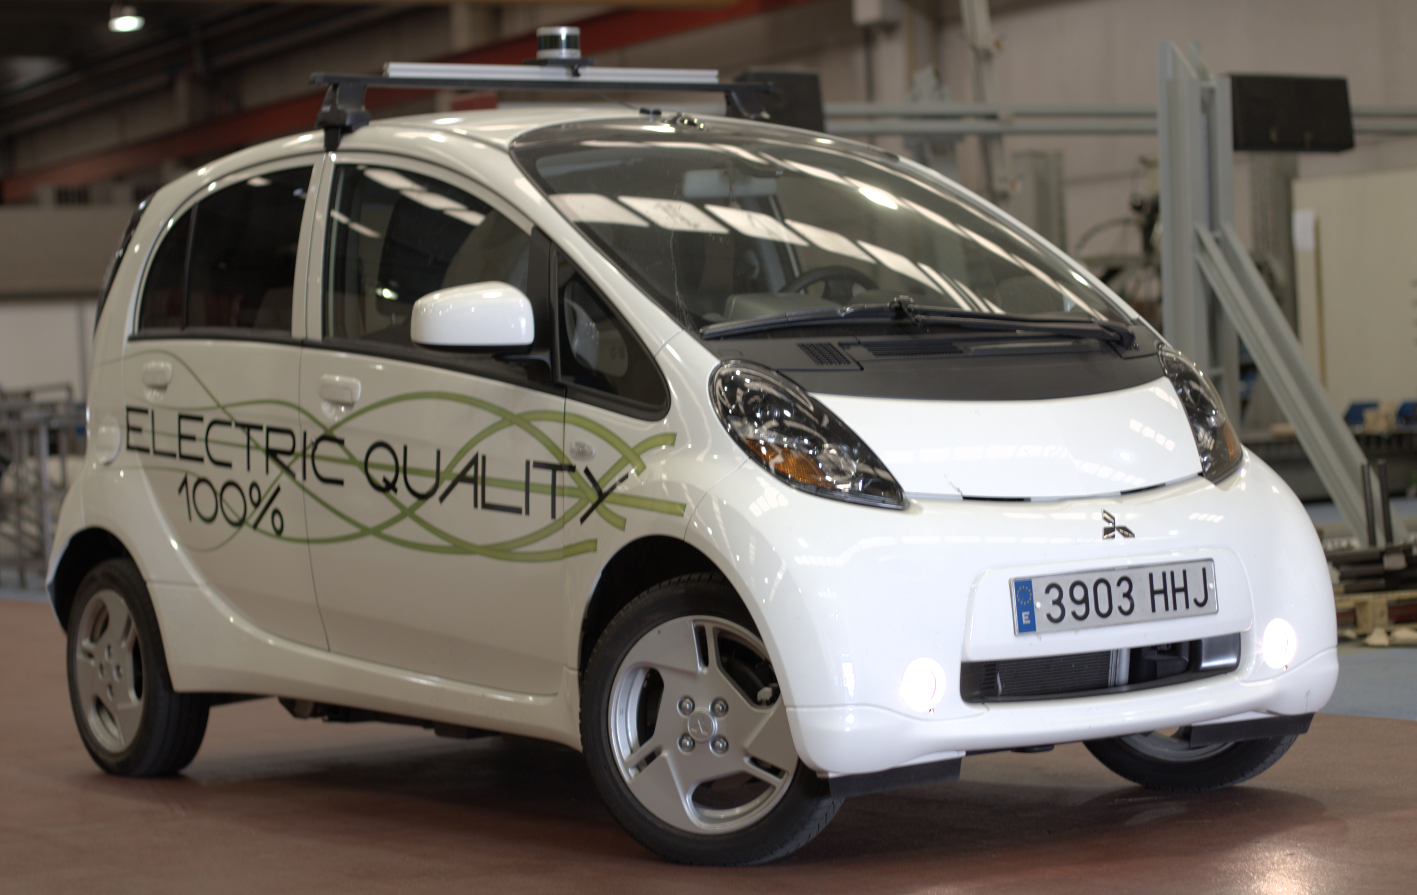
\includegraphics{instrumented-imiev}
	\caption{El vehículo utilizado en los ensayos realizados. Se trata de un Mitsubishi iMiEV instrumentado con un LIDAR anclado en la baca superior, un GPS anclado en el techo, un puerto de acceso directo al Bus CAN y una cámara Microsoft Kinect tras el espejo retrovisor.}
	\label{fig:instrumented-imievschema}
\end{figure}

\subsection{Dispositivos usados para la captura de datos}

A continuación se describen los dispositivos usados y su información generada.

\paragraph{\acrfull{lidar}}

Se trata de un dispositivo que usa uno o más haces de luz pulsada para el cálculo de la distancia a los objetos donde éstos impactan. Nuestro \ac{lidar} en concreto modelo VLP-16 de la empresa Velodyne.

Está compuesto por un único haz láser con un movimiento continuo vertical y horizontal capturando información con una apertura de campo vertical de \SI{\pm15}{\degree} distribuído a lo largo de 16 planos (dando como resultado una resolución fija de \SI{2}{\degree}), y un campo horizontal de visión de \SI{360}{\degree} con una resolución dependiente de la velocidad de giro del láser, de \SI{0.1}{\degree} a \SI{0.4}{\degree} para \SI{5}{\Hz} a \SI{20}{\Hz} respectivamente. Estas medidas permiten una captura desde $75000$ hasta $300000$ puntos del entorno en función de la velocidad de giro a una distancia de hasta \SI{100}{\meter}.

El acceso a la información se realiza a través del puerto Ethernet. Para la captura de datos se ha hecho uso del paquete de \ac{ros} destinado para el trabajo con estos dispositivos denominado \texttt{velodyne\_pointcloud}\sidenote{\url{http://wiki.ros.org/velodyne\_pointcloud}.}. Este nodo publica la nube de puntos en coordenadas cartesianas con el eje $X$ definido en el sentido de los \SI{0}{\degree} y el eje $Z$ en sentido ascendente.

\begin{marginfigure}
	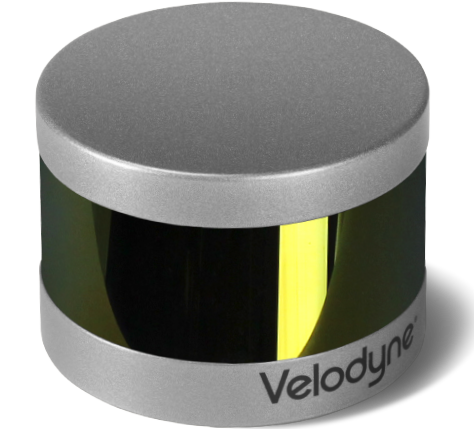
\includegraphics[width=\textwidth]{vlp-16}
	\caption{El \ac{lidar} VLP-16 de Velodyne tiene un FOV horizontal de \SI{360}{\degree} y vertical de \SI{\pm15}{\degree}, permitiendo una captura de todo el entorno circundante a una frecuencia de hasta \SI{20}{\Hz}. Fuente: \url{http://velodynelidar.com/vlp-16.html}.}
	\label{fig:vlp-16}
\end{marginfigure}

El \ac{lidar} instrumentado se encuentra anclado en la baca del vehículo con el eje $X$ dispuesto en el sentido de conducción y el eje $Z$ en sentido ascendente. Su posición es centrada en el vehículo y a una altura de \SI{1.75}{\meter}.

\paragraph{\ac{gps}}

El \ac{gps} es una tecnología usada para sincronización de tiempo y posicionamiento $3d$ (i.e. latitud, longitud y altitud) de objetos en el globo terráqueo. Es un dispositivo que funciona en un único sentido, es decir, el receptor recibe la información de los satélites, pero no envía ninguna.

El dispositivo \ac{gps} utilizado para los experimentos ha sido desarrollado en el Laboratorio de Electrónica e Instrumentación del \ac{insia}. Se trata de un dispositivo \ac{gps} con corrección diferencial que genera mensajes \ac{nmea} a una frecuencia de hasta \SI{20}{\Hz}. La posición de la antena receptora estará localizada en el centro del vehículo, justo debajo del \ac{lidar}, situándose de esta forma en el origen de coordenadas del entorno capturado con éste último.

\begin{marginfigure}
	\centering
	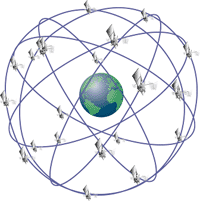
\includegraphics[width=\textwidth]{gps}
	\caption{El \ac{gps} permite el posicionamiento 3d sobre en la tierra gracias a la comunicación unidireccional de satélites situados en órbita. Fuente: Wikimedia Commons.}
	\label{fig:gps}
\end{marginfigure}

De todos los mensajes disponibles, los recuperados son lo de los siguientes tipos:

\begin{itemize}
	\item GGA. Geoposicionamiento del vehículo, el cual será usado para deducir valores no medibles directamente como, por ejemplo, la distancia al siguiente semáforo.
	\item VTG. Velocidad del vehículo, que se usará como el valor real de la velocidad tomada por el vehículo.
\end{itemize}

De la captura de datos se encargará el paquete de \ac{ros} denominado \texttt{nmea\_navsat\_driver} \sidenote{\url{http://wiki.ros.org/nmea\_navsat\_driver}.} el cual leerá por el puerto USB la información originada en el \ac{gps}.

\paragraph{Bus \acrfull{can}}

Un bus es una topología caracterizada por tener un único canal de comunicaciones donde los dispositivos se conectan, vierten la información y la reciben. El Bus \ac{can}, o simplemente \ac{can}, es un protocolo de comunicaciones basado en esta topología utilizado, entre otras muchas áreas, para la comunicación entre los diferentes dispositivos que componen un vehículo.

El estándar \ac{can} cubre únicamente las dos primeras capas del modelo \ac{osi}\sidenote{
	Las dos primeras capas son la capa física (la conexión el hardware a la red y la transmisión/recepción física de los datos) y la de enlace de datos (direccionamiento físico, detección de errores y control de flujo). Sobre el resto de niveles no existen un estándar definido y por tanto existen multiples protocolos de estas dependiendo del fabricante u organismo que lo implemente.
}, lo cual es suficiente para el acceso a la información del vehículo. Sin embargo, dependiendo del fabricante, los vehículo pueden contar con uno o más buses independientes, con acceso más o menos restringido y con identificadores de mensajes diferentes. Además, el acceso a esta información no suele ser accesible para el público general, por lo que lo normal es realizar una tarea previa de ingeniería inversa para identificar los mensajes correspondientes a los datos que se desean almacenar y su frecuencia.

\begin{marginfigure}
	\centering
	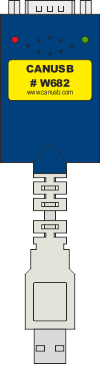
\includegraphics[width=.35\textwidth]{laciwel-canusb}
	\caption{El dispositivo CANBUS de LACIWEL AB permite el acceso a través del protocolo RS 232 por el puerto USB al bus \ac{can}. Fuente: \url{http://www.can232.com/}.}
	\label{fig:laciwel-canusb}
\end{marginfigure}

Del bus se ha recogido numerosa información, tanto para esta tesis como para más proyectos relacionados con ella. Para este experimento, no obstante, se ha utilizado únicamente la velocidad, y no directamente. La razón es que el \ac{can} ofrece ésta como un número entero, por lo que los cambios de velocidad durante los recorridos ocurren de \SI{\pm1}{\km\per\hour}. Esta resolución es insuficiente para los cálculos de la aceleración, por lo que se ha usado para validar la velocidad capturada por el \ac{gps}

El acceso a la información del bus se ha realizado a través del puerto USB. Para ello se ha utilizado el dispositivo CANUSB de la empresa LAWICEL AB, el cual se encarga de la traducción del protocolo CAN a una conexión estándar RS232. La captura de los paquetes se ha realizado a través de un nodo de \ac{ros} desarrollado para esta tesis.

\paragraph{Cámara}

Para la obtención de algunos valores de indicadores no existentes necesitamos un proceso posterior de análisis sobre el recorrido, asociando las imágenes a los valores recogidos del resto de dispositivos, como posiciones o nube de puntos del entorno. Para ello se ha hecho uso de una cámara para la visualización del recorrido desde el punto de vista del conductor.

La cámara utilizada es un Microsoft Kinect localizada tras el retrovisor interior del vehículo. Dicha cámara está orientada de tal manera que ofrece una visualización de la vía por la que circula el vehículo.

\begin{marginfigure}
	\centering
	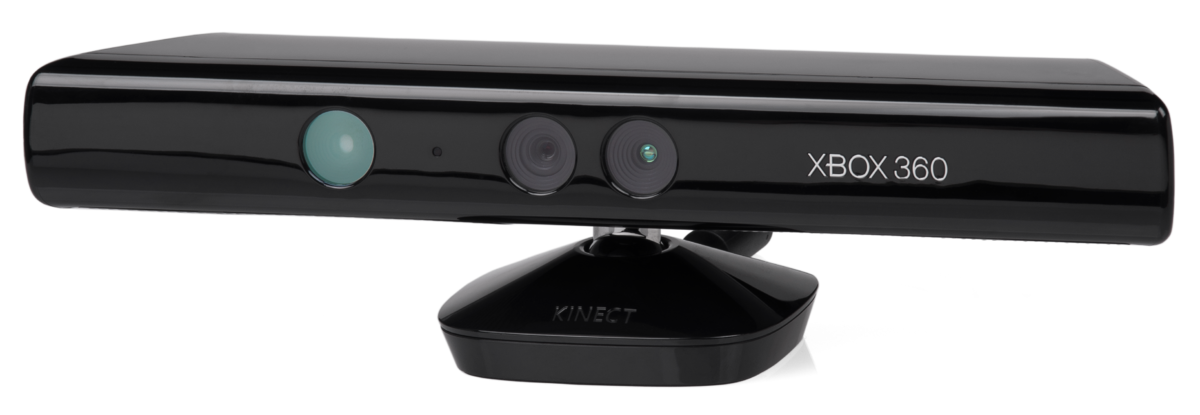
\includegraphics[width=\textwidth]{kinect}
	\caption{La cámara Kinect desarrollada por Microsoft ofrece imágenes a color a una velocidad de \SI{30}{\fps} con una resolución de \SI{640x480}{\px}.}
	\label{fig:kinect}
\end{marginfigure}

Entre otras capacidades, la cámara ofrece captura de imágenes VGA de \SI{640x480}{\px} de resolución y a una frecuencia de \SI{30}{\Hz}. El dispositivo se conecta vía USB y de la captura se encarga un nodo de ROS denominado \textit{freenect}\sidenote{\url{http://wiki.ros.org/freenect\_stack}.} 	que, entre otras cosas, public las imágenes tomadas a icha frecuencia.

\subsection{Selección de rutas}

Para la captura de datos se han propuesto dos rutas, en adelante $R_1$ y $R_2$, consideradas equivalentes al tratarse de vías en entorno urbano, con tramos de entre uno y tres carriles a lo largo de su recorrido y con velocidades máximas establecidas entre los \SI{30}{\km\per\hour} y los \SI{50}{\km\per\hour}. La figura~\ref{fig:proposed-routes} muestra los recorridos en el mapa.

$R_1$ tiene una duración de recorrido estimada de \SI{30}{\minute} y se utilizará como fuente de datos destinada al entrenamiento del modelo (conjuntos de entrenamiento y de validación). $R_2$ por su lado tiene un tiempo estimado de recorrido de \SI{15}{\minute} y sus datos tienen el propósito de servir de conjunto de test. Ambas fueron realizadas entre las 11:00am y las 12:00pm en días laborables, permitiendo una circulación con suficientes vehículos para requerir maniobras dependientes del entorno, pero sin demasiados como para impedir la circulación.

\begin{figure}[t]
	\centering
	\subfloat[]{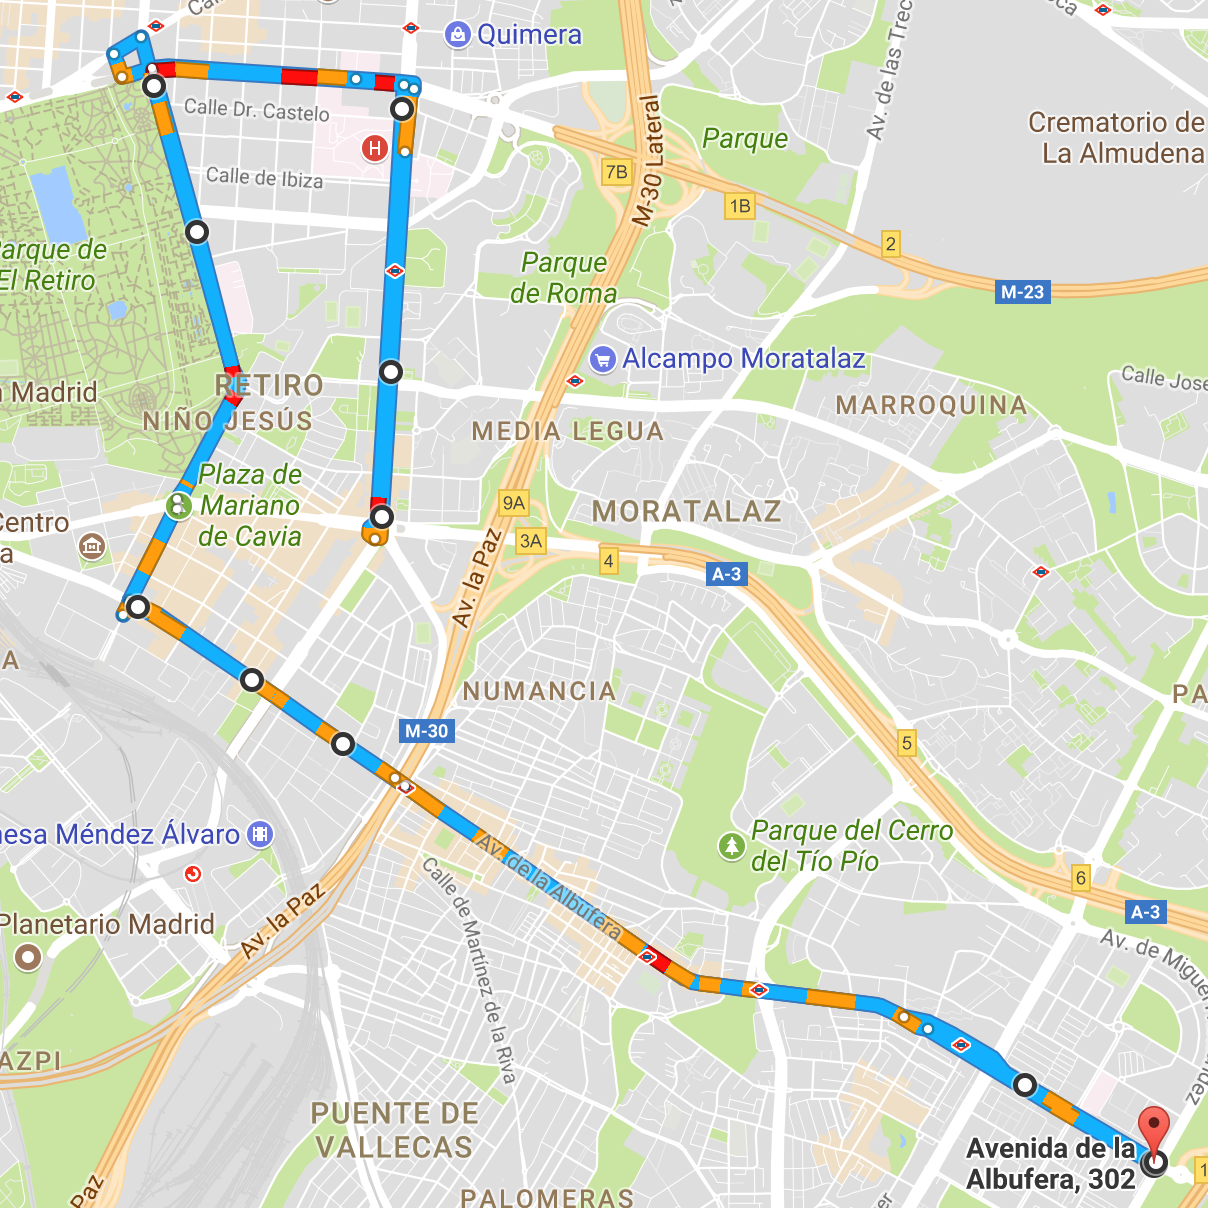
\includegraphics[width=.45\textwidth]{route-1}}\qquad
	\subfloat[]{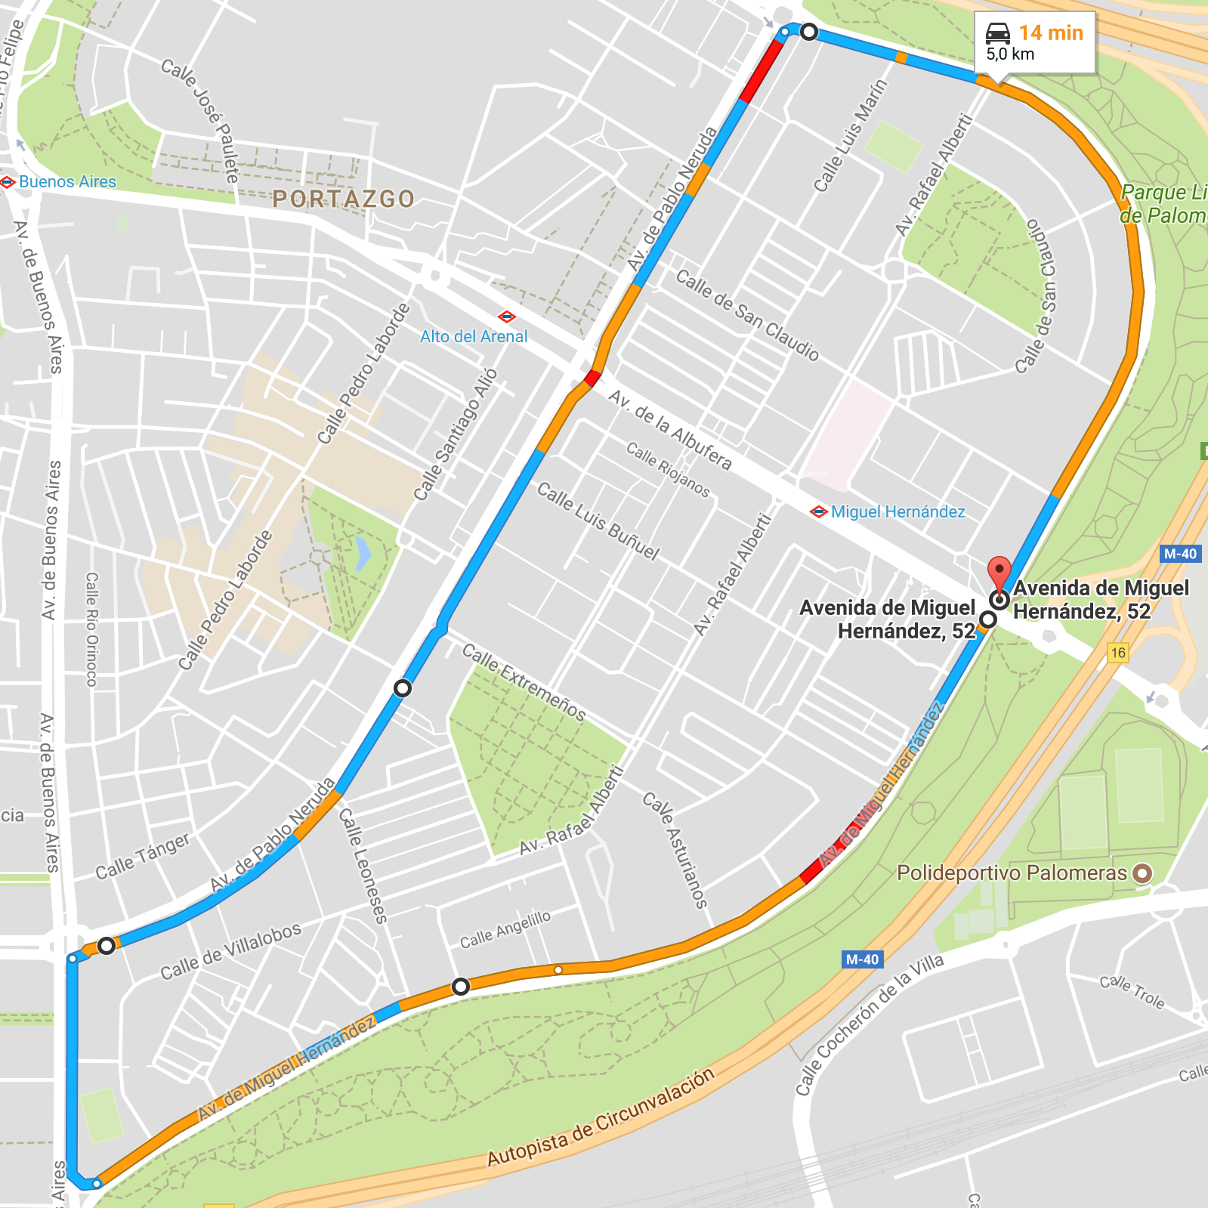
\includegraphics[width=.45\textwidth]{route-2}}
	\caption[Dos recorridos para la captura de datos de conducción]{Los dos recorridos realizados para la captura de datos de conducción, ambos en entorno urbano. (a) $R_1$ tiene una duración estimada de \SI{30}{\minute} y sirve para la captura de los datos de entrenamiento. (b) $R_2$ tiene una duración estimada de \SI{15}{\minute} y sus datos serán utilizdos para los conjuntos de test.\TODO{Poner la ruta de verdad}}
	\label{fig:proposed-routes}
\end{figure}

\subsection{Selección de sujetos}

Se han elegido un total de tres sujetos para los experimentos. Los tres pertenencen al grupo especificado en los supuestos del capítulo~\nameref{ch:intro}, es decir varones dentro del rango de $35$ a $39$ años.

Los sujetos tienen experiencia de conducción y han realizado el recorrido anteriormente a fin de basar sus comportamientos lo más posible al nivel táctico de conducción\sidenote{
	Dado que los comportamientos de \textit{car-following} y \textit{lane-change} se asocian con el nivel cognitivo táctico, se ha querido reducir el impacto del operador decidiendo durante el experimento hacia dónde o no ir. De esta manera los conductores son libres de realizar el movimiento que deseen y de anticipar maniobras con más libertad.
}.

\section{Preparación de los datos}

Tras la captura se ha realizado una secuencia de pasos para dejar los datos preparados para el proceso de entrenamiento de los modelos. El resto de la sección detalla cada uno de éstos.

\subsection{Fusión de sensores}

Como hemos visto anteriormente, cada uno de los dispositivos ofrece sus datos a una tasa de frecuencia diferente (con excepción del bus CAN, en el cual los datos van a frecuencias diferentes).

El primer paso en la preparación de los datos ha sido el de la fusión de estos. Afortunadamente cada uno de los mensajes almacenados que llegan desde nodos de ROS vienen con una marca temporal que podemos suponer sincronizada entre nodos de la misma aplicación. Por ello, la fusión se ha realizado en dos pasos:

\begin{enumerate}
	\item Cálculo del primer elemento a fusionar de cada uno de los conjuntos de datos. Para ello, se han desechado todos los primeros valores hasta encontrar la primera tupla de valores (uno por cada conjunto de datos) donde éstos están más próximos entre si.
	\item Extracción iterativa de las tuplas más aproximadas. Iterativamente, se han ido extrayendo las tuplas más próximas a cada uno de los incrementos de la tasa deseada de sincronización $f$, siempre y cuando se encuentren dentro del intervalo $f \pm \frac{f}{2}$.
\end{enumerate}

Este proceso se ha repetido con cada uno de los conductores para cada uno de los recorridos, dando como resultado seis conjuntos sincronizados con los datos en bruto sincronizados.

\subsection{Extracción de variables no observables directamente}

Existen una serie de variables cuya extracción directa del entorno no es trivial. Ésta es una de las razones por las que se ha capturado con la cámara la visión del conductor en el recorrido.

El proceso de obtenición ha sido manual, obteniendo las marcas temporales de las variables a capturar tras el visionado de las imágenes capturadas por la cámara. Estas variables son las siguientes:

\paragraph{Cambio de carril}

Se han identificado los cambios de carril, siendo estos marcados como $+1$ si es un cambio hacia la izquierda o $-1$ si es un cambio a la derecha, y por tanto, todos aquellos momentos en los que no hay cambio de carril se marcan tendrán un valor de $0$. Las marcas temporales de los cambios son aquellas desde el comienzo de la maniobra del cambio de carril hasta que el vehículo ha llegado a la mitad del cambio.

\paragraph{Velocidad máxima de la vía}

Se han añadido las velocidades máximas de las vías indicando las marcas temporales en las que el conductor entra o sale de cada uno de los tramos.

\paragraph{Distancia y estado de semáforos}

La distancia al semáforo ha sido obtenida a partir de la distancia euclídea entre la geoposición del origen de coordenadas y la geoposición del semáforo, por lo que es esperable cierto márgen de error. Los estados se han extraído directamente del visionado de las imágenes, tomando este los valores $g$, $y$ y $r$ dependiendo de si el semáforo se encuentra en verde, ámbar o rojo.

\paragraph{Distancia a recorrer en carriles}

Al igual que con la distancia a los semáforos, ésta se ha calculado a partir de la distancia euclídea de la geoposición del origen de coordenadas a los puntos a partir de los cuales no se puede continuar por el recorrido especificado.

Las distancias obtenidas se corresponden al carril izquiero, al actual y al derecho.

\paragraph{Distancia al obstáculo más cercano}

Para el cálculo de esta variable, se ha procedido a capturar una región de interés de cada una de las nubes de puntos dentro de la cual identificar los posibles obstáculos existentes. Por la posición del lidar se ha decidido que ésta está acotada entre los intervalos $(0.35, 35)$, $(-1, 1)$ y $(-1.5, 0.5)$ para los ejex X, Y y Z respectivamente.

Posteriormente, para la nube de puntos resultante se ha realizado un proceso de clusterización aplicando el algoritmo DBSCAN\sidenote{
	DBSCAN~\cite{ester1996density} es un algoritmo de clusterización que identifica un número variable de conjuntos en un espació $n$-dimensional.
	
	Funciona a partir de la agregación de puntos en función de sus parámetros $\epsilon$ y $\mu$. $\epsilon$ es la distancia mínima a la que se deben encontrar dos puntos para considerarse pertenecientes al mismo clúster mientras que $\mu$ determina el número mínimo de puntos que debe tener un clúster para ser considerado como tal.
} con parámetros $\epsilon = 0.5$ y $\mu = 3$. Este proceso identifica un número variable de clústers, tras el cual nos hemos quedado con el más cercando al vehículo.

Posteriormente y de forma manual, se ha realizado el recorrido mostrando las nubes de puntos correspondientes a las capturas superponiendo el centroide para eliminar los de aquellos frames que se corresponden con errores. De los restantes se ha calculado una distancia euclídea al origen de coordenadas.

\subsection{Curación de datos}

Tras obtener todas las variables principales, ya sean directamente de los sensores del coche o a través de un proceso manual generamos los conjuntos de datos para los comportamientos longitudinal y de cambio de carril. La tabla~\ref{tbl:main-variables} describe qué variables son usadas en qué conjunto de datos.

\begin{table}
	\centering
	\small
	\caption[Resumen de los indicadores obtenidos tras los recorridos]{Resumen de los indicadores obtenidos tras los recorridos. Éstos incluyen tanto la información extraída directamente como aquella que ha requerido proceso manual. La parte inferior de la tabla describe las variables a predecir en los problemas de modelo longitudinal y de cambio de carril. Las variables \enquote{Distancia circulable} en realidad es una tupla que indica las distancias circulables en los carriles izquierdo, actual y derecho.}
	\label{tbl:main-variables}
	\begin{tabular}{lcc}
		\toprule
		Variable & Longitudinal & Cambio de carril \\
		\midrule
		\rowcolor{black!20} Distancia circulable      & \nop & \yep \\
		Distancia al líder        & \yep & \nop \\
		\rowcolor{black!20} Distancia a siguiente TLS & \yep & \yep \\
		Estado de siguiente TLS   & \yep & \yep \\
		\rowcolor{black!20} Nube de puntos            & \nop & \yep \\
		Velocidad                 & \yep & \nop \\
		\rowcolor{black!20} Velocidad al líder        & \yep & \nop \\
		\midrule
		\textbf{Aceleración}      & \yep & \nop \\
		\rowcolor{black!20} \textbf{Cambio de carril} & \nop & \yep \\
		\bottomrule
	\end{tabular}
\end{table}

\section{Entrenamiento de modelos}

Para los entrenamientos de los modelos se ha utilizado una máquina con procesador Intel\textregistered Core\texttrademark i7-6700K a \SI{4.00}{\giga\Hz} y \SI{16}{\gibi\byte} de memoria. El sistema operativo utilizado ha sido un Debian GNU/Linux versión 9.4. 

Para cada uno de los submodelos se han probado dos aproximaciones diferentes para comparar sus desempeños en las tareas por separado. Concretamente se han utilizado \acp{fcs} y \acp{mlp} para modelar el comportamiento longitudinal y \acp{mlp} y \acp{cnn} para modelar el comportamiento en cambio de carril.

Los modelos serán entrenados con los conjuntos asociados al total de sujetos (esto es, $CT_{S_A}$ para el modelo longitudinal y $LT_{S_A}$ para el modelo de cambio de carril). Tras ello, y una vez decididos los modelos que se usarán para el modelo de conducción, se entrenarán dichas arquitecturas para los sujetos por separado.